\documentclass{article}
\usepackage[utf8]{inputenc}
\usepackage{graphicx}
\usepackage{amsmath}
\usepackage{amssymb}
\usepackage{amsthm}
\newcommand{\hide}[1]{}
\newcommand{\edit}[1]{\textcolor{red}{#1}}
\newtheorem{thm}{Theorem}
\newtheorem{lem}{Lemma}
\usepackage{xcolor}

\title{Shorter Superpatterns Using Compression}
\author{Zach Hunter}
\date{April 2020}

\begin{document}

\maketitle

\section{Introduction}


We say that $W_n$ is the set of maps $w:[n]\to [n]$, where $[n]:= \{1,2,\dots n\}$. These maps $w \in W_n$ are commonly thought of as being words of length $n$ on the alphabet $[n]$. We say $w \in W_n$ contains another word $w' \in W_k$, and write $w' \in w$, if there are indices $1 \le  x_1 < \dots  < x_k \le  n$ such that for $1 \le i, j \le k$ we have $w(x_i) < w(x_j)$ if and only if $w'(i)<w'(j)$. We denote $S_n$ as the set of bijections $\pi:[n]\to[n]$, and say a word $w$ is $k$-universal or a $k$-superpattern if it contains every $\pi \in S_k$.


Now, let $F(k)$ denote the minimum $n$ such that there exists a $k$-superpattern $w \in W_n$. For convenience, we introduce $f(k) :=\frac{F(k)}{k^2}$ as a normalized version of $F$. In 1999, Arratia observed that $f(k) \ge 1/e^2+o(1)$ by Stirling's approximation, and conjectured that $f(k) \le 1/e^2+o(1)$ also held. This was disproved by Chroman et al. who proved $f(k) \ge 1.000076/e^2 +o(1)$. \hide{https://arxiv.org/abs/2004.02375v1}

In 2007, Eriksson et al., it was proven that $f(k)\le 2/3+o(1)$, and conjectured that $f(k) \ge 1/2+o(1)$. \hide{(H. Eriksson, K. Eriksson, S. Linusson, and J. Wästlund, Dense packing of patterns in a
permutation, Ann. Comb. 11 (2007), no. 3-4, 459–470.)}
In 2009, it was shown that $f(k) \le 1/2+o(1)$ by Miller, and in 2018 Engen and Vatter slightly improved  $o(1)$ term for this.\hide{A. Miller, Asymptotic bounds for permutations containing many different patterns, J. Combin.
Theory Ser. A 116 (2009), no. 1, 92–108.} \hide{Michael Engen and Vincent Vatter. Containing all permutations. 2018. arXiv: 1810.08252 [math.CO].} In this paper, we prove:

\begin{thm}
There exists $k$-superpatterns of length $\frac{15}{32}k^2 +O(k)$.
\end{thm}Thus, we get that $f(k) \le 15/32+o(1)$ refuting the conjecture of Eriksson et al.. \edit{clean summary of past results}


\section{Preliminaries}

\textbf{Abuse of Notation:} Throughout this paper, $[a,b]$ will be shorthand for the set of positive integers $x$ such that $a \le x \le b$.

We start by introducing a lemma, which was stated as Proposition 5.2 in a paper by Engen and Vatter, and was inspired by the proof of Theorem 3.1 in Miller's paper.

Define zigzag. Define $w_+$.

\begin{lem}

\end{lem}

We shall recap the proof provided by Engen and Vatter, to establish some ideas that shall also be used in proving our main result.

Give their proof.

We can now describe our proof. Without affecting the asymptotics, we shall only concern ourselves with constructing $k$-superpatterns where $k$ is divisible by $4$. Throughout the rest of this paper, will let $m = k/4$.

We will first define a zigzag-like word which has an alphabet of $3(m+3)$ letters.

We will first define a map $\phi:[4m]\to [3m]$ which will ``compress'' our alphabet. In particular, for integers $i$, we will have $\phi([4i+1,4(i+1)]) =[3i+1,3(i+1)]$, which will us to use a divide-and-conquer-type approach to the decompression process.

\section{Compression}



\section{Decompression}

We address the case where $n = 4m$.

Let $\phi$ be a map that sends $x = 4k+i \to (k,i-\lfloor i/3\rfloor)$, where $i \in \{1,2,3,4\}$. For each permutation on $n$-letters, $\pi$, we derive a new word, $p$ where $p(i) = \phi(\pi(i))$. We then create the word $q$ by removing all immediate repetitions in in $p$. (e.g. if $p = 2,1,1,2,3,3$, then $q = 2,1,2,3$)

Let $z_{m+1}$ be the zigzag word restricted to $[m+1]$. We create a new zigzag word, $z_{m+1}'$, by replacing each even integer $x$ with the letters $(x,1),(x,2),(x,3)$, and each odd integer $y$ with the letters $(y,3),(y,2),(y,1)$.

Let $q^\oplus$ be the word obtained replacing each letter $(k,i)$ with the letter $(k+1,i)$. By the same argument as in result 5.2, we have $w(q)+w(q^\oplus) = 1$, since the parity of each letter swaps and order in each parity does not change. (by parity, we mean whether $k$ is even/odd for each letter $(k,i)$)

We will now define an order on $z_{m+1}'$, $\zeta_{m+1}'$. Suppose $z_{m+1}'(a) = (k_1,i_1)$ and $z_{m+1}'(b) = (k_2,i_2)$. If $k_1 > k_2$, we say $\zeta_{m+1}'(a) > \zeta_{m+1}'(b)$. If $k_1 = k_2$ and $i_1 > i_2$, then $\zeta_{m+1}'(a) > \zeta_{m+1}'(b)$. 

Otherwise $z_{m+1}'(a) = z_{m+1}'(b) = (k,i)$. Let $f(x)$ count the number of appearances of $(k,i)$ in the first $x$ letters $z_{m+1}'$. If $i <3$, then $\zeta_{m+1}'(a) > \zeta_{m+1}'(b)$ if $\frac{(-1)^{f(a)+i}}{f(a)} > \frac{(-1)^{f(b)+i}}{f(b)}  $. If $i = 3$, then $\zeta_{m+1}'(a) > \zeta_{m+1}'(b)$ if $f(a)(-1)^k > f(b)(-1)^k$.

Pictorally, here is how $\zeta'$ would be ordered restricted to the letters $(2,1),(2,2),(2,3)$:


\begin{figure}[htp]
    \centering
    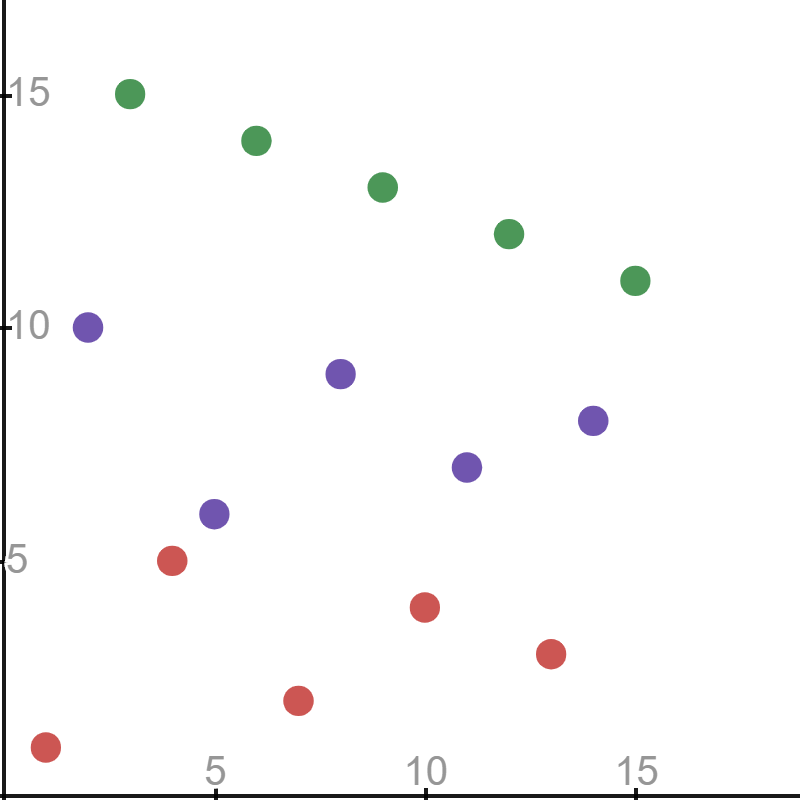
\includegraphics[width=4cm]{desmos-graph}
    \caption{Red dots are the letter (2,1), purple dots are (2,2), and green are (2,3).}
\end{figure}

Meanwhile, restricting to $(1,1),(1,2),(1,3)$ we get:

\begin{figure}[htp]
    \centering
    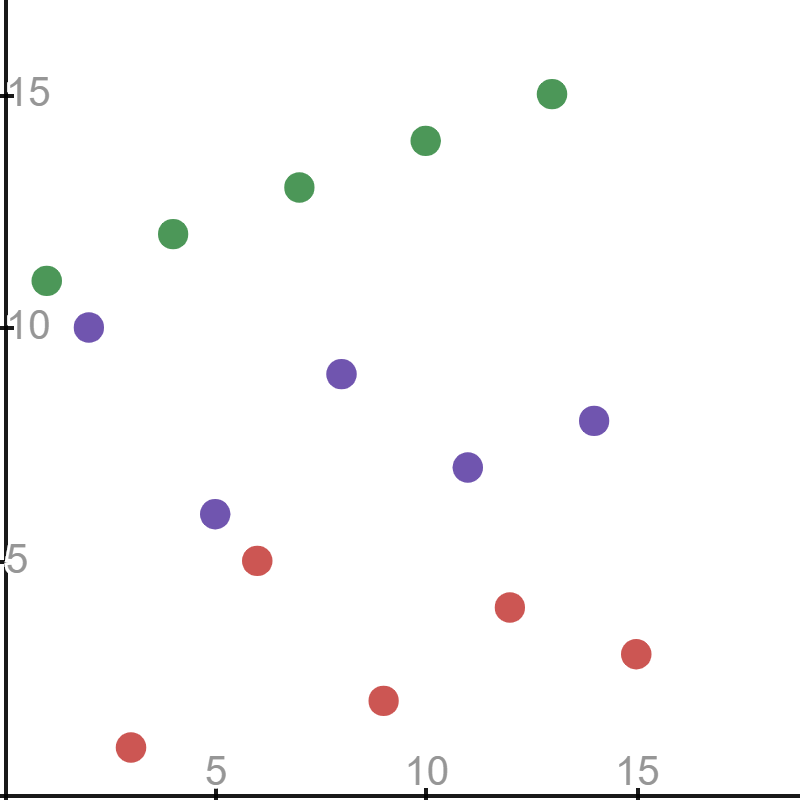
\includegraphics[width=4cm]{desmos-graph (1)}
    \caption{Red dots are the letter (1,1), purple dots are (1,2), and green are (1,3).}
\end{figure}

Note how red and purple alternate oppositely in the same run. Meaning, in $j$-th run, if the red letter is larger than all subsequent red letters, the purple is smaller than all subsequent purple letters. Conversely, if red is small, then purple is big.

The only other thing to note is that green is ascending for one parity, and descending in the other.

We now want to take the embeddings of $q$ and $q^\oplus$ to get proper order-isomorphic subsequences $a,b$ in $\zeta_{m+1}'$, where $w(a)+w(b)\ge n/2 + 1$. We do this by running through the current embeddings, and tweak them in a way which is not affected by future tweaks, such that the each set of letters $4k+1,4k+2,4k+3,4k+4$ are in the right order, and where the worst case net change of weight is 2 per set.

Case 1: $4k+2$ is not in the way

If $4k+4$ appears before $4k+3$, then $(k,3)$ and $(k,2)$ appear in different runs when $k$ has even parity. Thus, have assumed $4k+2$ is not in the way, we are allowed to move $4k+3$ up to the top row to get a correct order with cost zero for the even parity. Conversely, if $4k+3$ appears after $4k+3$, then we can move $4k+3$ up to the top row to get a correct order with cost zero for the odd parity. 

Thus, we are left to handle the remaining parity. Here, we cannot possibly move $4k+3$ to the top row. 


Subcase 1.1: $4k+2$ and $4k+3$ are in different runs.

If the order between $4k+2$ and $4k+3$ is incorrect, then shifting things ahead to the next run fixes it, within the desired cost. Otherwise, the order was already fine and we are done anyways.

Subcase 1.2: $4k+2$ and $4k+3$ were adjacent in $\pi$.

In $q$ and $q^\oplus$, the expanding adds two letters, decreasing bet weight by 2, meaning we now can use cost 4. Do one shift to expand, and then one two fix order if necessary.

Case 2: $4k+2$ is in the way.

i.e. if $4k+4$ comes before $4k+3$, then $4k+2$ is immediately after $4k+2$ and shares their run.

For the good parity of case 1, we first shift expand, and then move $4k+3$ up. This costs 2. Thus, we are left with cost 2 for the other side.

In the remaining parity, $4k+3$ will be first in its run. If $4k+1$ is not also in the run, then we can push $4k+2$ down, and then shift if need be to fix order between $4k+1$ and $4k+2$.

Thus, we may assume they are all in the same run. If the middle is at a peak, then we may shift $4k+2$ and $4k+1$ together to achieve order. Otherwise, the bottom is a peak, meaning we can push $4k+2$ down, and shift $4k+1$ over, and are done.


\iffalse
Let's just address the case where $n = 4k$. Let $z_{2k+2}$ be the zigzag word restricted to $[2k+2]$.

Let $\phi:\Bbb{Z} \to \Bbb{Z}$ be the map where $\phi(x+8) = \phi(x) +4$ and $\phi(1) = \phi(2) = 1, \phi(3) = \phi(4) = 3, \phi(5) = \phi(6) = 2, \phi(7) = \phi(8) = 4$. 

For each permutation on $n$-letters, $\pi$, we derive a new word, $p$ where $p(i) = \phi(\pi(i))$. We then create the word $q$ by removing all immediate repetitions in in $p$. (e.g. if $p = 2,1,1,2,3,3$, then $q = 2,1,2,3$)

Let $q^\oplus$ be the word obtained by increasing the values odd letters by 1 and values of even letters by 3.* By the same argument as in result 5.2, we have $w(q)+w(q^\oplus) = 1$, since the parity of each letter swaps and order in each parity does not change.

*The reason why we use $q^\oplus$ instead of $q^+$ is that this ``preserves pairs'', meaning that if $q(i)$ and $q(j)$ are in the same part, $p$, of the partition $\mathcal{P} = \{ \{1,3\}, \{2,4\},\{5,7\},\dots\}$, then $q^\oplus(i)$ and $q^\oplus(j)$ will both be in some part $p' \in \mathcal{P}$.

We now wish to modify $z_{2k+2}$. We wish to pair up consecutive letters in each run. Here, $2,4,6,8,10,12$ would become $(2,4),(6,8),(10,12)$. In between each pair, we insert a new letter. (so, $(2,4),(6,8),(10,12)$ would become $2,a_{2,4},4, 6,a_{6,8},8,10,a_{10,12},12$) Imposing the changes, we have a new word $Z_{2k+2}$. 

We impose a new order $\prec$ upon $Z_{2k+2}$. Suppose $Z_{2k+2}(i) = \ell = Z_{2k+2}(j)$, with $i < j$. If $\ell$ is an integer, we ``alternate'' the ordering. Let $f(x)$ count the number of appearances of $\ell$ in the first $x$ letters $Z_{2k+2}$. We then say that $Z_{2k+2}(i) \prec Z_{2k+2}(i)$ if and only if $f(i)(-1)^{f(i)} < f(j)(-1)^{f(j)}$.

If $\ell = a_{x,x+2}$, and $x$ is even, then $Z_{2k+2}(i) \succ Z_{2k+2}(j)$. Conversely, if $\ell = a_{x,x+2}$, and $x$ is odd, we say $Z_{2k+2}(i) \prec Z_{2k+2}(j)$. This handling of parity is not arbitrary, and is chosen based off the fact that even runs in $z_n$ ascend, $2,4,\dots$, while odd runs descend, $\dots, 5,3,1$.

Meaning, if $a^i$ is the $i$-th appearance of $a_{x,x+1}$, then $a^i \prec a^j \iff i(-1)^i < j(-1)^j$.

Finally, having established how we break ties between repetition of letters, we lastly say that $1\prec a_{1,3} \prec 3 \prec 2 \prec a_{2,4} \prec 4 \prec 5 \prec a_{5,7} \dots$. With this in place, if $x< y$ and $\phi(x) \neq \phi(y)$, then $\phi(x) \prec \phi(y)$ according to this ordering.

It follows that the embeddings of $q$ and $q^\oplus$ into $z_{2k+2}$ correspond to embeddings almost order-isomorphic to $\pi$ in $\zeta_{2k+2}$, where we just need to expanded repeats, and fix the ordering between consecutive numbers.

Let $q_0$ and $q^\oplus_0$ be the embeddings in $\zeta_{2k+2}$ derived from the embeddings of $q$ and $q^\oplus$ in $z_{2k+2}$. Let $q_i$ loosely mean, a modified embedding of $q_{i-1}$ into $\zeta_{2k+2}$ where we fixed the ordering of $4i+1,4i+2,4i+3,4i+4$ to match their order found in $\pi$. We will show that in the worst case, that we have  $w(q_i)+w(q_i^\oplus) \leq w(q_{i-1})+w(q_{i-1}^\oplus)+2$. 

Let us now more accurately define $q_i$, and what the worst case cost means. We have that $q_0$ embed $x$ into $\phi(x)$, and this will not change until we fix the ordering of $x$. 

Thus, letting $X = \phi(4i+1)$, we have that $q_{i-1}$ embed $4i+1$ and $4i+2$ into $X$, and embed $4i+3$ and $4i+4$ into $X+2$.

We then choose a word $W_i \in \{X,a_{X,X+2},X+2\}^4$, such that there is an embedding of $W_i$ in $\zeta_{2k+2}$ that is order isomorphic to the restriction of $\pi$ to $4i+1,4i+2,4i+3,4i+4$. Our choice of $W_i$ shall only depend on the restriction of $\pi$ to $4i+1,4i+2,4i+3,4i+4$. With the words $W_1,W_2\dots W_i$, we construct $q_i$ from $q_0$.

TO EXPLAIN MORE FORMALLY: Basically replace letters according to $W_i$, i.e. if $W_1 = 1, 3, a_{1,3}, a_{1,3}$, then we'd replace the $t$-th appearance of a letter in $\{1,3\}$ with $W_1(t)$, and place two letters on top of one another if they where a repeat removed by $q$. Then, starting from first letter in our modified embedding, if two letters are on top of another, or if we need to change the parity of $a_{x,x+2}$ to correct the ordering, we move all letters that have left in our embedding ahead two runs. We define $w(W_i)$ to be the most the weight should change by implementing $W_i$ if parities change maliciously.

Thus, more accurately, instead of the worst case cost $w(q_i)$, we actually mean the weaker, but more predictable upper bound, $w(q_0) + \sum_1^i w(W_i)$, where $w(W_i)$ is the worst-case weight change for implement $W_i$.


We handle the case of $q^\oplus_i$ in the same fashion. Since $q^\oplus_i$ has different parity, this changes how ties are broken when embedding into $X'$ and $X'+2$. We shall show that $w(W_i(\pi))+w(W_i(\pi^\oplus)) \le 2$.

If this is true, then $w(q_n)+w(q_n^\oplus) \le 1+2(n/4) = 1+n/2$, which implies that either $q_n$ or $q_n^\oplus$ can be embedded with weight $n/4$, which takes $5n/4$ runs. Thus, we can embed any $\pi$ into a word with $(2k+2)/2(3/2)(5n/4) = \frac{15n^2}{32} +\frac{15n}{8}$ letters.

Hence, we are left to address the various cases in which $4i+1,4i+2,4i+3,4i+4$ could get embedded by $q_0$, depending on our choice of $\pi$. The relevent information is, the order of $4i+1,4i+2,4i+3,4i+4$ according to $\pi$, whether there any repeats, in $p(\pi)$ that are removed from $q$, and what letters are in the same run. 

This leads to there being 100 different cases.  We can easily eliminate 24 cases, for when there are no repetitions, and all letters are in different runs. TO COMPLETE 
\fi
\end{document}
